% Inbuilt themes in beamer
\documentclass{beamer}
\usepackage{minted}
\usepackage{amsmath}
\usepackage{amsfonts}

% Title page details: 
\title{Dimensionality Reduction} 
\author{Ammar, Callum, Lewis, Skye}
\date{\today}


\begin{document}

% Title page frame
\begin{frame}
    \titlepage 
\end{frame}

% Remove logo from the next slides
\logo{}


% Outline frame
\begin{frame}{Outline}
    \tableofcontents
\end{frame}


% Unassigned
\section{Introduction}
\begin{frame}{Introduction}

\end{frame}

% Lewis
\section{Linear Methods}
\subsection{PCA}
\begin{frame}{Principle Component Analysis}
\end{frame}

% Ammar
\section{Non-linear Methods}
\subsection{UMAP}
\begin{frame}{Uniform Manifold Approximation and Projection}
    
\end{frame}

\subsection{t-SNE}
\begin{frame}{T-Distributed Stochastic Neighbor Embedding}
    
\end{frame}

\section{Interpretable Dimensionality Reduction}
\subsection{NMF}
\begin{frame}{Non-Negative Matrix Factorization}
    
\end{frame}

\section{Deep Learning Methods}
\subsection{Autoencoders}
\begin{frame}{Autoencoder}
    Given an input space $\mathcal{X} \equiv \mathbb{R}^n$ and a target low dimension space $\mathcal{Z} \equiv \mathbb{R}^d$, $d \ll n$, learn two parameterised functions $d_\theta$ and $e_\phi$ such that
    \begin{align*}
        x \approx d_\theta(e_\phi(x)) && e_\phi(x) \in \mathcal{Z}.
    \end{align*}
\end{frame}

\subsection{VAE}
\begin{frame}{Variational Autoencoder}
    Let $d_\theta$ and $e_\phi$ define distributions over $\mathcal{X}$ and $\mathcal{Z}$ respectively and define a prior $p$ over $\mathcal{Z}$.\\~\\

    The models can be trained by maximizing
    \begin{equation*}
        \mathbb{E}_{z \sim e_\phi(\cdot;x)}\left[\ln\frac{d_\theta(x;z)p(z)}{e_\phi(z;x)}\right]
    \end{equation*}
    for all $x$ in the training set.\\~\\

    The expectation is known as the evidence lower-bound.
\end{frame}

\begin{frame}{Variational Autoencoder}
    \begin{figure}
        \centering
        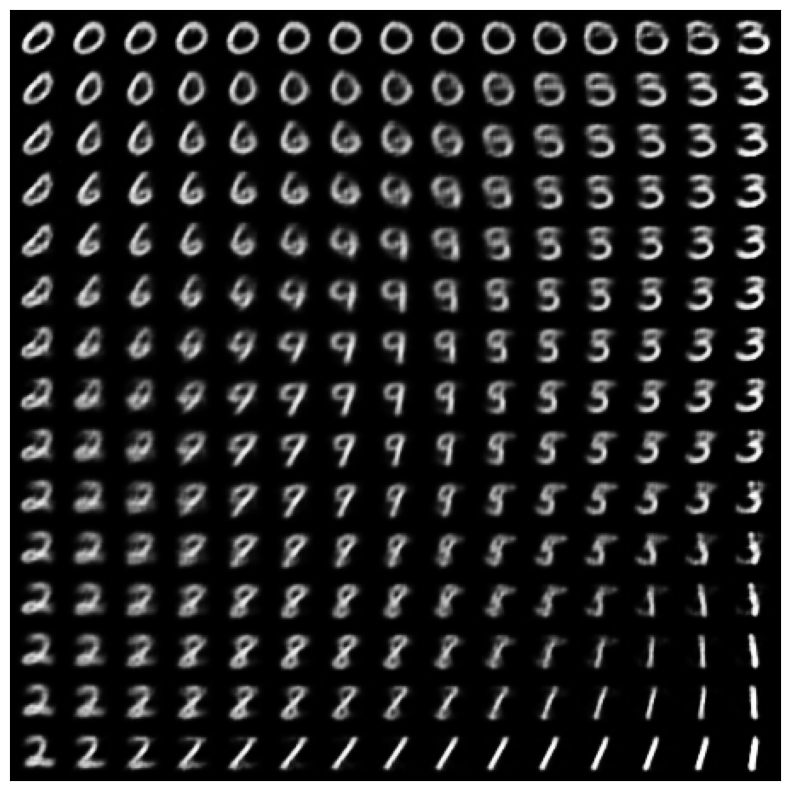
\includegraphics[width=0.5\linewidth]{vae.png}
        \caption{Visualisation of MNIST latent space with latent dimension 2.}
        \label{fig:vae}
    \end{figure}
\end{frame}

\begin{frame}[fragile]
    \frametitle{Variational Autoencoder}
    \begin{minted}{python}
        class Encoder:
            ...
            def forward(self, x):
                mu, sigma = self.encode(x)
                return Normal(mu, sigma)

        class Decoder:
            ...
            def forward(self, z):
                p_x = self.decode(z)
                return Bernoulli(p_x)
    \end{minted}
\end{frame}

\begin{frame}[fragile]
    \frametitle{Variational Autoencoder}
    \begin{minted}[xleftmargin=0.7mm]{python}
        def train(data, enc, dec, ...):
            prior = Normal(0,1)
            ...
            for x in data:
                posterior = enc(x)
                z_sample = posterior.sample()
                
                log_prior = prior.log_prob(z_sample)
                log_posterior = posterior.log_prob(
                    z_sample)
                log_lik = dec(z_sample).log_prob(x)

                loss = -(
                    log_prior.sum(1) +
                    log_posterior.sum(1) -
                    log_lik.sum(1,2,3)
                ).mean()
                loss.backward()
                ...
    \end{minted}
\end{frame}

\end{document}